\documentclass[a4paper,11pt]{report}
\usepackage{chuan_math_gkt}
\usetikzlibrary{angles,quotes,intersections,patterns,decorations.pathreplacing}
\chuanexamsetup

\begin{document}
\examfontsize

\examsecret{绝密$\bigstar$启用前}

\examtitle{2025年普通高等学校招生全国统一考试（新高考I卷）}{数\quad 学}

\noticetitle
\begin{examnotice}
\item 答卷前，考生务必将自己的姓名、准考证号填写在答题卡上. 
\item 回答选择题时，选出每小题的答案后，用铅笔把答题卡上对应题目的答案标号涂黑. 如需改动，用橡皮擦干净后，再选涂其他答案标号. 回答非选择题时，将答案写在答题卡上. 写在本试卷上无效. 
\item 考试结束后，将本试卷和答题卡一并交回. 
\end{examnotice}

\examsection{一、选择题：本大题共8小题，每小题5分，共计40分. 每小题给出的四个选项中，只有一个选项是正确的. 请把正确的选项填涂在答题卡相应的位置上. }
\begin{examquestions}
\item $(1+5\mathrm{i})\mathrm{i}$ 的虚部为
\fourchoices{$-1$}{$0$}{$1$}{$6$}
\item 设全集 $U=\{x\mid x\text{是小于9的正整数}\}$，集合 $A=\{1,3,5\}$，则 $\complement_UA$ 中元素个数为
\fourchoices{$0$}{$3$}{$5$}{$8$}
\item 若双曲线 $C$ 的虚轴长为实轴长的 $\sqrt7$ 倍，则 $C$ 的离心率为
\fourchoices{$\sqrt2$}{$2$}{$\sqrt7$}{$2\sqrt2$}
\item 若点 $(a,0)(a>0)$ 是函数 $y=2\tan\left(x-\dfrac\pi3\right)$ 的图象的一个对称中心，则 $a$ 的最小值为
\fourchoices{\tallchoice{$\dfrac\pi6$}}{\tallchoice{$\dfrac\pi3$}}{\tallchoice{$\dfrac\pi2$}}{\tallchoice{$\dfrac{4\pi}{3}$}}
\item 设 $f(x)$ 是定义在 $\mathbb R$ 上且周期为2的偶函数，当 $2\leq x\leq3$ 时，$f(x)=5-2x$，则 $f\left(-\dfrac34\right)=$
\fourchoices{\tallchoice{$-\dfrac12$}}{\tallchoice{$-\dfrac14$}}{\tallchoice{$\dfrac14$}}{\tallchoice{$\dfrac12$}}
\clearpage
\item 帆船比赛中，运动员可借助风力计测定风速的大小和方向，测出的结果在航海学中称为视风风速，视风风速对应的向量，是真风风速对应的向量与船行风速对应的向量之和，其中船行风速对应的向量与船速对应的向量大小相等，方向相反. 图1给出了部分风力等级、名称与风速大小的对应关系. 已知某帆船运动员在某时刻测得的视风风速对应的向量与船速对应的向量如图2（风速的大小和向量的大小相同），单位（$\mathrm{m/s}$），则真风为

\begin{tightcenter}
\begin{minipage}[c]{0.43\linewidth}
\centering
\renewcommand{\arraystretch}{1.45}
\begin{tabular}{|c|c|c|}
\hline
等级 & 风速大小 $\mathrm{m/s}$ & 名称 \\
\hline
2 & $1.1\sim3.3$ & 轻风 \\
\hline
3 & $3.4\sim5.4$ & 微风 \\
\hline
4 & $5.5\sim7.9$ & 和风 \\
\hline
5 & $8.0\sim10.1$ & 劲风 \\
\hline
\end{tabular}

\vspace{0.4em}
图1
\end{minipage}
\hspace{1.0cm}
\begin{minipage}[c]{0.36\linewidth}
\centering
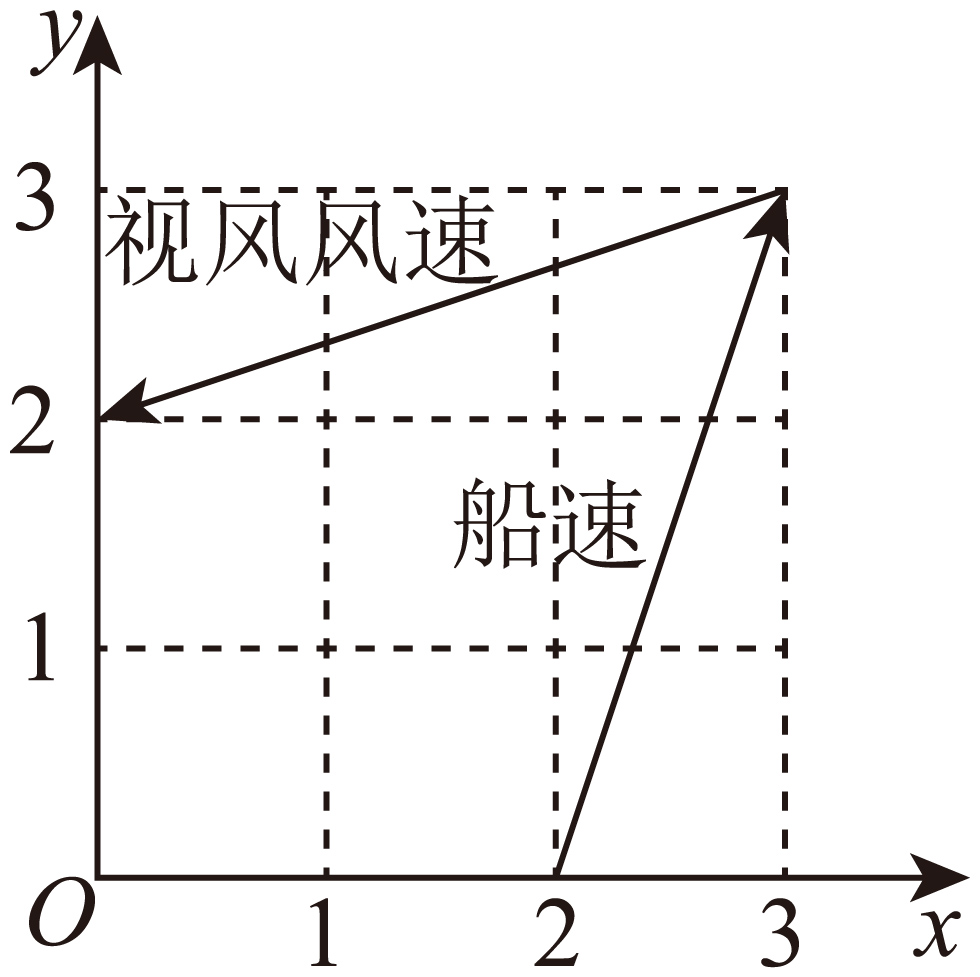
\includegraphics[width=4.1cm]{figures/2025_xgk1_q6.png}

\vspace{0.4em}
图2
\end{minipage}
\end{tightcenter}

\fourchoices{轻风}{微风}{和风}{劲风}
\item 若圆 $x^2+(y+2)^2=r^2(r>0)$ 上到直线 $y=\sqrt3x+2$ 的距离为1的点有且仅有2个，则 $r$ 的取值范围是
\fourchoices{$(0,1)$}{$(1,3)$}{$(3,+\infty)$}{$(0,+\infty)$}
\item 若实数 $x,y,z$ 满足 $2+\log_2x=3+\log_3y=5+\log_5z$，则 $x,y,z$ 的大小关系不可能是
\twochoices{$x>y>z$}{$x>z>y$}{$y>x>z$}{$y>z>x$}
\end{examquestions}
\examsection{二、选择题：本题共3小题，每小题6分，共18分. 在每小题给出的选项中，有多项符合题目要求. 全部选对的得6分，部分选对的得部分分，有选错的得0分. }
\begin{examquestions}[start=9]
\item 在正三棱柱 $ABC-A_1B_1C_1$ 中，$D$ 为 $BC$ 中点，则
\twochoices{$AD\perp A_1C$}{$BC\perp$ 平面 $AA_1D$}{$CC_1\parallel$ 平面 $AA_1D$}{$AD\parallel A_1B_1$}
\item 设抛物线 $C:y^2=6x$ 的焦点为 $F$，过 $F$ 的直线交 $C$ 于 $A,B$，过 $F$ 且垂直于 $AB$ 的直线交 $l:x=-\dfrac32$ 于 $E$，过点 $A$ 作准线 $l$ 的垂线，垂足为 $D$，则
\twochoices{$|AD|=|AF|$}{$|AE|=|AB|$}{$|AB|\geq6$}{$|AE|\cdot|BE|\geq18$}
\newpage
\item 已知 $\triangle ABC$ 的面积为 $\dfrac14$，若 $\cos^2A+\cos^2B+2\sin C=2$，$\cos A\cos B\sin C=\dfrac14$，则
\twochoices{$\sin C=\sin^2A+\sin^2B$}{$AB=\sqrt2$}{$\sin A+\sin B=\dfrac{\sqrt6}{2}$}{$AC^2+BC^2=3$}
\end{examquestions}
\examsection{三、填空题：本大题共3小题，每小题5分，共计15分. }
\begin{examquestions}[start=12]
\item 若直线 $y=2x+5$ 是曲线 $y=e^x+x+a$ 的切线，则 $a=\blank$. 
\item 若一个等比数列的前4项和为4，前8项和为68，则该等比数列的公比为\blank. 
\item 一个箱子里有5个相同的球，分别以1～5标号，若每次取一颗，有放回地取三次，记至少取出一次的球的个数 $X$，则数学期望 $E(X)=\blank$. 
\end{examquestions}
\examsection{四、解答题：本题共5小题，共77分. 解答应写出文字说明、证明过程或演算步骤. }
\begin{examanswers}[start=15]
\item（13分）

为研究某疾病与超声波检查结果的关系，从做过超声波检查的人群中随机调查了1000人，得到如下列联表：
\begin{tightcenter}
\begin{tabular}{|c|c|c|c|}
\hline 超声波检查结果组别 & 正常 & 不正常 & 合计\\ \hline
患该疾病 & 20 & 180 & 200\\ \hline
未患该疾病 & 780 & 20 & 800\\ \hline
合计 & 800 & 200 & 1000\\ \hline
\end{tabular}
\end{tightcenter}
\subq{（1）}{记超声波检查结果不正常者患该疾病的概率为 $P$，求 $P$ 的估计值；}

\subq{（2）}{根据小概率值 $\alpha=0.001$ 的独立性检验，分析超声波检查结果是否与患该疾病有关. 
附：$\chi^2=\dfrac{n(ad-bc)^2}{(a+b)(c+d)(a+c)(b+d)}$. 
\begin{tightcenter}
\begin{tabular}{|c|c|c|c|}
\hline $P(\chi^2\geq k)$ & 0.005 & 0.010 & 0.001\\ \hline
$k$ & 3.841 & 6.635 & 10.828\\ \hline
\end{tabular}
\end{tightcenter}
\newpage
}
\item（15分）

设数列 $\{a_n\}$ 满足 $a_1=3$，$\dfrac{a_{n+1}}{n}=\dfrac{a_n}{n+1}+\dfrac1{n(n+1)}$. 

\subq{（1）}{证明：$\{na_n\}$ 为等差数列；}

\subq{（2）}{设 $f(x)=a_1x+a_2x^2+\cdots+a_mx^m$，求 $f'(-2)$.}
\item（15分）

如图所示的四棱锥 $P-ABCD$ 中，$PA\perp$ 平面 $ABCD$，$BC\parallel AD$，$AB\perp AD$. 

\noindent\begin{minipage}[t]{0.64\linewidth}
\subq{（1）}{证明：平面 $PAB\perp$ 平面 $PAD$；}

\subq{（2）}{$PA=AB=\sqrt2$，$AD=1+\sqrt3$，$BC=2$，$P,B,C,D$ 在同一个球面上，设该球面的球心为 $O$.}

\subq{（i）}{证明：$O$ 在平面 $ABCD$ 上；}

\subq{（ii）}{求直线 $AC$ 与直线 $PO$ 所成角的余弦值.}
\end{minipage}\hfill
\begin{minipage}[t]{0.30\linewidth}
\vspace{-0.6em}
\centering
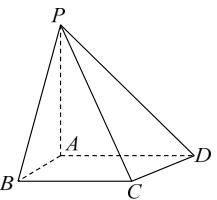
\includegraphics[width=\linewidth]{figures/2025_xgk1_q17.png}
\end{minipage}
\item（17分）

设椭圆 $C:\dfrac{x^2}{a^2}+\dfrac{y^2}{b^2}=1(a>b>0)$ 的离心率为 $\dfrac{2\sqrt2}{3}$，下顶点为 $A$，右顶点为 $B$，$|AB|=\sqrt{10}$. 

\subq{（1）}{求椭圆的标准方程；}

\subq{（2）}{已知动点 $P$ 不在 $y$ 轴上，点 $R$ 在射线 $AP$ 上，且满足 $|AR|\cdot|AP|=3$.}

\subq{（i）}{设 $P(m,n)$，求点 $R$ 的坐标（用 $m,n$ 表示）；}

\subq{（ii）}{设 $O$ 为坐标原点，$M$ 是椭圆上的动点，直线 $OR$ 的斜率为直线 $OP$ 的斜率的3倍，求 $|PM|$ 的最大值.}
\item（17分）

\subq{（1）}{设函数 $f(x)=5\cos x-\cos5x$，求 $f(x)$ 在 $\left[0,\dfrac\pi4\right]$ 的最大值；}

\subq{（2）}{给定 $\theta\in(0,\pi)$，设 $a$ 为实数，证明：存在 $y\in[a-\theta,a+\theta]$，使得 $\cos y\leq\cos\theta$；}

\subq{（3）}{若存在 $\varphi$ 使得对任意 $x$，都有 $5\cos x-\cos(5x+\varphi)\leq b$，求 $b$ 的最小值.}
\end{examanswers}

\end{document}
